\documentclass{article}
\usepackage{verbatim}
\usepackage{fullpage}
\usepackage{amsmath}
\usepackage{graphicx}
\usepackage{listings}
\usepackage{placeins} % for \FloatBarrier
%% package for contiued float
\usepackage{caption}
\usepackage[english,greek, main=greek]{babel}
\usepackage[utf8]{inputenc}
\useshorthands{;}
\defineshorthand{;}{?}

\usepackage{pythonhighlight}

\usepackage[explicit]{titlesec} % number after section name
%% the following lines are used to reset the section counter
%% after 'part' is encountered.
\makeatletter
\@addtoreset{section}{part}
\makeatother
%% the following lines are used to add the section number
%% after the section name
\titleformat{\section}
  {\normalfont\large\bfseries}
  {}
  {0em}
  {#1\ \thesection}
%% number after subsection name
\titleformat{\subsection}
  {\normalfont\large\bfseries}
  {}
  {0em}
  {#1\ \thesubsection}
%% avoid numbering contents
\titleformat{\section}
  {\normalfont\Large\bfseries}
  {}
  {0em}
  {\ifnum\value{section}=0\relax #1\else #1\ \thesection\fi}
\newcommand{\eng}[1]{\foreignlanguage{english}{#1}} % shortcut for inserting english into greek text


\title{
    \includegraphics[width=\textwidth]{~/Pictures/emp.png} \\
    \vskip 5cm
    Νευροασαφής Έλεγχος και Εφαρμογές\\
    \large Άσκηση 3η
    \vskip 5cm
}

\author{Αναστάσιος Στέφανος Αναγνώστου\\
        03119051}

\begin{document}

\maketitle
\newpage
\tableofcontents
\newpage

\part{Αλγόριθμοι Βελτιστοποίησης}

Αρχικά, για όλες τις ασκήσεις του μέρους αυτούς, γράφηκαν κατάλληλες
συναρτήσεις που υλοποιούν τους διαφόρους αλγορίθμους βελτιστοποίησης.
Παρατίθενται όλες εδώ:

\selectlanguage{english}
\begin{python}
import numpy as np 

def gradient_descent(f, df, x_curr, a, eps=0.001, limit=1000):
    value = f(*x_curr)
    delta = df(*x_curr)
    x_next = x_curr - a * delta 
    nvalue = f(*x_next)
    iterations = 0
    while abs(value - nvalue) > eps and iterations < limit:
        value = nvalue
        delta = df(*x_next)
        x_next = x_next - a * delta 
        nvalue = f(*x_next)
        iterations += 1
    return nvalue, x_next, iterations

def newtons_method(f, df, ddf, x_curr, a, eps=0.001, limit=1000):
    x_next = x_curr - df(*x_curr) / ddf(*x_curr)
    value = f(*x_curr)
    nvalue = f(*x_next)
    iterations = 0
    while abs(value - nvalue) > eps and iterations < limit:
        value = nvalue
        x_next += -df(*x_next) / ddf(*x_next)
        nvalue = f(*x_next)
        iterations += 1
    return nvalue, x_next, iterations

def momentum_method(f, df, x_curr, a1, a2, eps=0.001, limit=1000):
    v_curr = np.array([0, 0])
    v_next = a1 * v_curr - a2 * df(*x_curr)
    x_next = x_curr + v_next
    iterations = 0;
    while abs(f(*x_curr) - f(*x_next)) > eps and iterations < limit:
        v_curr = v_next
        x_curr = x_next
        v_next = a1 * v_curr - a2 * df(*x_curr)
        x_next = x_curr + v_next
        iterations += 1;
    return f(*x_next), x_next, iterations
\end{python}
\selectlanguage{greek}

\clearpage
\section{Θέμα}

Εξετάζεται η σύγκλιση του αλγορίθμου \eng{gradient descent} για την εύρεση του
ελαχίστου της συνάρτησης $f(x_1,x_2) = x_1^2 +(x_2 - 1)^2 + (x_1 - x_2)^4$, για
τα διάφορα μεγέθη βήματος.

\selectlanguage{english}
\begin{python}
def f(x1, x2):
    return x1**2 + (x2 - 1)**2 + (x1 - x2)**4

def df(x1, x2):
    return np.array([2*x1 + 4*(x1 - x2)**3, 2 *(x2 - 1) - 4*(x1 - x2)**3])

def ddf(x1, x2):
    return (4 + 24*(x1 - x2)**2)

if __name__ == '__main__':
    np.set_printoptions(precision=3)
    steps = [0.1 - 0.01 * i for i in range(0, 10)]
    initial = np.array([2, 5])
    for step in steps:
        minimum, minimizer, loops = gradient_descent(f, df, initial, step)
    steps = [0.1 + 0.1 * i for i in range(0, 10)]
    for step in steps:
        minimum, minimizer, loops = newtons_method(f, df, ddf, initial, step)
\end{python}
\selectlanguage{greek}

Το αποτέλεσμα της προσομοίωσης φαίνεται παρακάτω.

\selectlanguage{english}
\begin{verbatim}
========= ========= gradient descent ========= =========
step = 0.100: inf, [-4.109e+298  4.109e+298], 5
step = 0.090: inf, [-1.112e+280  1.112e+280], 5
step = 0.080: inf, [-9.334e+258  9.334e+258], 5
step = 0.070: inf, [-3.826e+234  3.826e+234], 5
step = 0.060: inf, [ inf -inf], 6
step = 0.050: inf, [ inf -inf], 6
step = 0.040: inf, [ inf -inf], 6
step = 0.030: inf, [-inf  inf], 7
step = 0.020: 0.199, [0.326 0.826], 89
step = 0.010: 0.211, [0.359 0.859], 163
========= ========= newton's method  ========= =========
step = 0.100: 0.189, [0.276 0.776], 24
step = 0.200: 0.189, [0.276 0.776], 24
step = 0.300: 0.189, [0.276 0.776], 24
step = 0.400: 0.189, [0.276 0.776], 24
step = 0.500: 0.189, [0.276 0.776], 24
step = 0.600: 0.189, [0.276 0.776], 24
step = 0.700: 0.189, [0.276 0.776], 24
step = 0.800: 0.189, [0.276 0.776], 24
step = 0.900: 0.189, [0.276 0.776], 24
step = 1.000: 0.189, [0.276 0.776], 24
\end{verbatim}
\selectlanguage{greek}

Φαίνεται ότι ο αλγόριθμος \eng{gradient descent} δεν συγκλίνει για μεγάλα βήματα
και ότι ο αλγόριθμος \eng{Newton} συγκλίνει, ανεξαρτήτως του μεγέθους του βήματος,
στο ίδιο ελάχιστο και με το ίδιο πλήθος επαναλήψεων.

\clearpage
\section{Θέμα}

Για τον υπολογισμό του \eng{condition number} της παράστασης $f(x1, x2) = A
\cdot x_1^2 + \frac{1}{A} \cdot x_2^2$, γράφτηκε ο παρακάτω κώδικας σε
\eng{Python}.

\selectlanguage{english}
\begin{python}
def f(x1, x2, A=10):
    return A*x1**2 + (1/A)*x2**2
def df(x1, x2, A=10):
    return np.array([2*A*x1, (2/A)*x2])
def ddf(x1, x2, A=10): # not actually a function of x1, x2
    return 2*A + (2/A)
if __name__ == '__main__':
    As = [1.2*i for i in range(1, 11)]
    initial = np.array([50, -100]) # initial guess for the minimizer
    for A in As:
        min, minimizer, loops = gradient_descent(lambda x1, x2: f(x1, x2, A),
                                                 lambda x1, x2: df(x1, x2, A),
                                                 initial, 0.05)
        cond = max(2*A, 2/A)/min(2*A, 2/A) # condition number of hessian
    for A in As:
        min, minimizer, loops = momentum_method(lambda x1, x2: f(x1, x2, A),
                                                lambda x1, x2: df(x1, x2, A),
                                                initial, 0.5, 0.05)
        cond = max(2*A, 2/A)/min(2*A, 2/A)
\end{python}
\selectlanguage{greek}

Παρατίθενται τα αποτελέσματα των δύο αλγορίθμων βελτιστοποίησης για τις
διάφορες τιμές του Α. Σε κάθε γραμμή φαίνεται το Α, το \eng{condition number},
η ελάχιστη τιμή, το σημείο ελαχιστοποίησης και ο αριθμός των επαναλήψεων.

\selectlanguage{english}
\begin{verbatim}
========= ========= gradient descent ========= =========
A = 1.200, Cond num = 1.440: 0.004, [ 0.001 -0.073], 82
A = 2.400, Cond num = 5.760: 0.011, [ 5.033e-17 -1.618e-01], 150
A = 3.600, Cond num = 12.960: 0.017, [ 2.602e-40 -2.478e-01], 212
A = 4.800, Cond num = 23.040: 0.023, [ 5.443e-76 -3.328e-01], 270
A = 6.000, Cond num = 36.000: 0.029, [ 9.344e-129 -4.173e-001], 325
A = 7.200, Cond num = 51.840: 0.035, [ 1.485e-208 -4.988e-001], 378
A = 8.400, Cond num = 70.560: 0.041, [ 0.    -0.587], 428
A = 9.600, Cond num = 92.160: 0.047, [ 0.   -0.67], 477
A = 10.800, Cond num = 116.640: 0.053, [ 0.    -0.757], 524
A = 12.000, Cond num = 144.000: 0.059, [ 0.    -0.841], 570
\end{verbatim}
\selectlanguage{greek}

Κάτι που παρατηρείται είναι ότι όσο αυξάνεται το \eng{condition number} του
πίνακα \eng{Hessian} τόσο αυξάνεται και ο αριθμός των επαναλήψεων που
απαιτούνται για την σύγκλιση του αλγορίθμου \eng{gradient descent}.

\selectlanguage{english}
\begin{verbatim}
========= ========= momentum method  ========= =========
A = 1.200, Cond num = 1.440: 0.001, [ 0.001 -0.03 ], 31
A = 2.400, Cond num = 5.760: 0.004, [-4.210e-10 -1.028e-01], 71
A = 3.600, Cond num = 12.960: 0.008, [-3.105e-15 -1.653e-01], 105
A = 4.800, Cond num = 23.040: 0.010, [ 2.768e-20 -2.222e-01], 137
A = 6.000, Cond num = 36.000: 0.013, [-2.347e-24 -2.819e-01], 167
A = 7.200, Cond num = 51.840: 0.016, [ 1.103e-28 -3.383e-01], 196
A = 8.400, Cond num = 70.560: 0.019, [-1.113e-33 -4.040e-01], 223
A = 9.600, Cond num = 92.160: 0.022, [ 5.048e-37 -4.607e-01], 250
A = 10.800, Cond num = 116.640: 0.025, [ 1.095e-40 -5.195e-01], 276
A = 12.000, Cond num = 144.000: 0.028, [-6.123e-45 -5.813e-01], 301
\end{verbatim}
\selectlanguage{greek}

Φαίνεται ότι ο αλγόριθμος \eng{momentum method} είναι πιο αποδοτικός από τον
αλγόριθμο \eng{gradient descent}. Αν και για μικρά \eng{condition numbers} οι
δύο αλγόριθμοι βρίσκουν κοντινά ελάχιστα, όσο αυτοί αυξάνονται ο αλγόριθμος
\eng{gradient descent} αρχίζει να αποκλίνει από την ελάχιστη τιμή.
Ο δε αλγόριθμος \eng{momentum method} παραμένει σταθερός και βρίσκει την
ελάχιστη τιμή, μάλιστα σε μικρότερο αριθμό επαναλήψεων.

\clearpage
\section{Θέμα}

Εξετάζεται ο \eng{condition number} του πίνακα $Q = A \cdot A^T$ όπου $A$ είναι
τυχαίος πίνακας, σαν συνάρτηση της διάστασης του $A$. Για κάθε διάσταση
παράγεται ένας αριθμός τυχαίων πινάκων και υπολογίζεται ο μέσος όρος των
\eng{condition numbers}. Ο μέσος όρος μπορεί να υπολογιστεί με πολλούς τρόπους,
παραδείγματος χάριν, ως αριθμητικός μέσος όρος ή ως αρμονικός μέσος όρος. Ο
κώδικας επιδεικνύει τον υπολογισμό του αριθμητικού μέσου όρου, όμως στα
αποτελέσματα παρουσιάζονται περισσότεροι.

\selectlanguage{english}
\begin{python}
import numpy as np
if __name__ == '__main__':
    cond_numbers = []
    reps = 400
    for dim in range(2, 100):
        cond_list = []
        for i in range(reps):
            A = np.random.randn(dim, dim)
            Q = A @ A.T
            cond = np.linalg.cond(Q)
            cond_list.append(cond)
        # use arithmetic mean
        mean_cond = np.mean(cond_list)
        cond_numbers.append(mean_cond)
\end{python}
\selectlanguage{greek}

Τα δε αποτελέσματα της προσομοιώσης εώς και 100 διαστάσεις φαίνονται παρακάτω.

\begin{figure}[h]
    \centering
    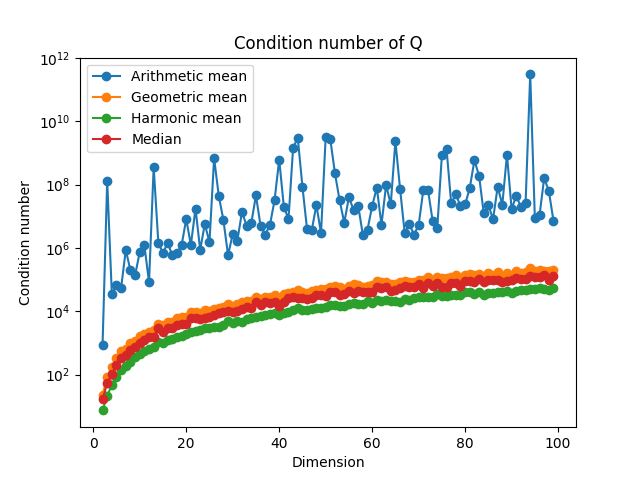
\includegraphics[width=0.8\textwidth]{part1/condition_number_vs_dims.png}
    \caption{Υπολογισμός \eng{condition number}}
\end{figure}

\clearpage
\section{Θέμα}

\selectlanguage{english}
\begin{python}
from optimizers import gradient_descent
from numdifftools import Gradient
import numpy as np

def f(x1, x2):
    return max(x1 + x2,
               0.9*x1 - 1.1*x2 + 1,
               -0.8*x1 + 1.2*x2 -1,
               2 - 1.1*x1 - 0.9*x2)

def df(x1, x2):
    return Gradient(f)(x1, x2)

if __name__ == '__main__':
    step = 0.001 # the optimization oscillates if the step is not small enough
    for _ in range(20):
        guess = np.array([np.random.uniform(5), np.random.uniform(5)])
        minimum, minimizer, loops = gradient_descent(f, df, guess, step, limit=10000)
\end{python}
\selectlanguage{greek}

Παρακάτω φαίνονται τα αποτελέσματα της προσομοίωσης. Σε κάθε γραμμή τυπώνονται με την σειρά:
Το ελάχιστο που βρέθηκε, το σημείο ελαχιστοποίησης, ο αριθμός επαναλήψεων και το σημείο εκκίνησης.
Το βήμα για τα παρακάτω αποτελέσματα είναι $0.01$.

\selectlanguage{english}
\begin{verbatim}
1.080 [-0.243  1.319] 345 [3.154 4.716]
2.052 [ 0.441 -0.596] 316 [3.411 2.374]
1.097 [-0.39  1.48] 147 [1.058 2.929]
1.049 [0.051 0.994] 136 [1.379 2.322]
2.313 [ 0.415 -0.854] 370 [3.942 2.673]
2.543 [ 0.393 -1.081] 272 [2.938 1.464]
4.481 [ 0.2   -3.001] 510 [4.876 1.675]
2.636 [ 0.383 -1.174] 310 [3.265 1.708]
1.881 [ 0.458 -0.426] 382 [4.14  3.256]
1.041 [0.225 0.816] 91 [1.124 1.715]
1.953 [1.54  0.394] 159 [3.14  1.994]
1.081 [-0.249  1.325] 189 [1.609 3.183]
1.055 [0.025 1.03 ] 273 [2.744 3.749]
1.030 [0.309 0.701] 391 [4.229 4.621]
1.048 [0.096 0.952] 293 [3.026 3.881]
3.676 [ 0.282 -2.203] 389 [3.889 1.404]
3.022 [ 0.346 -1.555] 369 [3.822 1.921]
3.441 [ 0.304 -1.971] 394 [3.919 1.644]
2.790 [ 0.368 -1.326] 359 [3.679 1.985]
1.256 [0.808 0.429] 204 [2.858 2.479]
\end{verbatim}
\selectlanguage{greek}

Φαίνεται ότι υπάρχει διακύμανση στο ελάχιστο που βρίσκεται από τον αλγόριθμο, καθώς και στο πλήθος
των επαναλήψεων που απαιτήθηκαν. Αυτό οφείλεται στο γεγονός ότι η συνάρτηση υπό ελαχιστοποίηση δεν είναι
ομαλή, με αποτέλεσμα να ταλαντώνεται ο βελτιστοποιητής. Ωστόσο, το πλήθος των απαιτούμενων επαναλήψεων
είναι γενικά λίγο.

Το βήμα για τα παρακάτω αποτελέσματα είναι $0.001$.

\selectlanguage{english}
\begin{verbatim}
1.065 [-0.077  1.143] 1684 [1.607 2.827]
1.353 [0.92  0.431] 1389 [2.31  1.821]
1.008 [0.458 0.549] 1531 [1.989 2.08 ]
2.217 [-0.278  2.495] 1572 [1.294 4.067]
1.040 [0.159 0.88 ] 3776 [3.935 4.656]
3.328 [2.993 0.333] 1914 [4.908 2.248]
1.307 [0.871 0.434] 2174 [3.046 2.608]
1.010 [0.452 0.558] 1600 [2.052 2.158]
1.975 [1.572 0.401] 1687 [3.26  2.089]
1.005 [0.501 0.504] 2307 [2.808 2.811]
1.089 [-0.313  1.402] 3555 [3.242 4.957]
1.019 [0.362 0.657] 4156 [4.518 4.813]
2.382 [2.001 0.38 ] 701 [2.703 1.082]
1.565 [-0.343  1.908] 2102 [1.759 4.01 ]
1.022 [0.343 0.679] 3512 [3.855 4.191]
1.887 [-0.311  2.198] 2775 [2.464 4.973]
2.270 [-0.272  2.543] 1565 [1.293 4.108]
2.767 [2.404 0.361] 1403 [3.807 1.764]
1.208 [0.768 0.439] 2349 [3.118 2.789]
1.015 [0.41  0.604] 4161 [4.571 4.765]
\end{verbatim}
\selectlanguage{greek}

Με πιο μικρό βήμα η τιμή του ελαχίστου παρουσιάζει μικρότερη διακύμανση, αναμενόμενο αφού
οι ταλαντώσεις λόγω της μη ομαλότητας της συνάρτησης ελαττώνονται, αλλά αυξάνονται κατά πολύ
οι επαναλήψεις που απαιτούνται για την σύγκλιση.

\clearpage
\section{Θέμα}

Για την συνάρτηση $f(x_1, x_2) = \frac{1}{4} \sum_{i=1}^{4} (x_1 - a_i)^2 + (x_2 - b_i)^2$,
όπου $a_i, b_i$ είναι τυχαίοι αριθμοί, εξετάζεται η σύγκλιση του αλγορίθμου
\eng{gradient descent} και του αλγορίθμου \eng{stochastic gradient descent}.
Σε κάθε επανάληψη, για την μέθοδο \eng{stochastic gradient descent} υπολογίζεται
τυχαία ένα από τα $d_i = \frac{1}{2} [x_1 - a_i, x_2 - b_i]^T$. Παρακάτω φαίνεται
ο κώδικας που χρησιμοποιήθηκε για την προσομοίωση.

\selectlanguage{english}
\begin{python}
def f(x1, x2, alphas, betas):
    return 1/4*(sum((x1-a)**2 + (x2-b)**2 for a, b in zip(alphas, betas)))
def df(x1, x2, alphas, betas):
    return 1/2 * np.array([sum(x1-a for a in alphas), sum(x2-b for b in betas)])
def df_sample(x1, x2, alphas, betas):
    a, b = random.choice(list(zip(alphas, betas)))
    return 1/2 * np.array([x1 - a, x2 - b])
if __name__ == '__main__':
    step = 0.1
    alphas = [random.randint(0, 10) for _ in range(4)]
    betas = [random.randint(0, 10) for _ in range(4)]
    loops_stoch, loops_ord = [], []
    for _ in range(10):
        guess = np.array([np.random.uniform(10), np.random.uniform(10)])
        minimum, minimizer, loops = gradient_descent(
                lambda x1, x2: f(x1, x2, alphas, betas),
                lambda x1, x2: df_sample(x1, x2, alphas, betas),
                guess, step)
        loops_stoch.append(loops)
        minimum, minimizer, loops = gradient_descent(
                lambda x1, x2: f(x1, x2, alphas, betas),
                lambda x1, x2: df(x1, x2, alphas, betas),
                guess, step)
        loops_ord.append(loops)
    avg_loops_ord = sum(loops_ord)/len(loops_ord)
    avg_loops_stoch = sum(loops_stoch)/len(loops_stoch)
\end{python}
\selectlanguage{greek}

Παρακάτω φαίνονται τα αποτελέσματα της προσομοίωσης.

\selectlanguage{english}
\begin{verbatim}
minimum | minimizer | iterations | initial guess | method
19.899 | [5.12  3.666] | 305    | [3.799 2.956] | stochastic
19.876 | [5.217 3.732] | 16     | [3.799 2.956] | ordinary
19.880 | [5.317 3.777] | 192    | [6.055 6.649] | stochastic
19.876 | [5.259 3.783] | 19     | [6.055 6.649] | ordinary
19.888 | [5.315 3.843] | 849    | [3.184 9.013] | stochastic
19.877 | [5.235 3.789] | 21     | [3.184 9.013] | ordinary
19.913 | [5.221 3.942] | 714    | [4.028 7.039] | stochastic
19.877 | [5.236 3.788] | 19     | [4.028 7.039] | ordinary
19.917 | [5.094 3.617] | 207    | [2.149 3.325] | stochastic
19.876 | [5.214 3.745] | 19     | [2.149 3.325] | ordinary
19.892 | [5.337 3.652] | 132    | [9.772 4.865] | stochastic
19.876 | [5.283 3.758] | 21     | [9.772 4.865] | ordinary
19.945 | [5.237 4.014] | 88     | [5.863 9.751] | stochastic
19.876 | [5.254 3.785] | 22     | [5.863 9.751] | ordinary
19.891 | [5.313 3.859] | 83     | [2.857 5.658] | stochastic
19.876 | [5.222 3.772] | 19     | [2.857 5.658] | ordinary
19.922 | [5.354 3.558] | 882    | [1.393 1.018] | stochastic
19.876 | [5.222 3.73 ] | 21     | [1.393 1.018] | ordinary
19.889 | [5.191 3.854] | 49     | [8.818 2.579] | stochastic
19.876 | [5.283 3.739] | 20     | [8.818 2.579] | ordinary
average number of iterations (stochastic) = 350.1
average number of iterations (ordinary) = 19.7

minimum | minimizer | iterations | initial guess | method
5.892 | [7.855 2.825] | 103     | [6.77  1.729] | stochastic
5.877 | [7.722 2.721] | 15      | [6.77  1.729] | ordinary
5.883 | [7.839 2.744] | 61      | [2.56 7.68] | stochastic
5.876 | [7.725 2.773] | 23      | [2.56 7.68] | ordinary
5.883 | [7.825 2.795] | 70      | [6.867 5.15 ] | stochastic
5.876 | [7.737 2.785] | 18      | [6.867 5.15 ] | ordinary
5.914 | [7.925 2.839] | 94      | [3.291 4.417] | stochastic
5.876 | [7.717 2.762] | 21      | [3.291 4.417] | ordinary
5.889 | [7.819 2.845] | 196     | [6.801 8.635] | stochastic
5.876 | [7.744 2.785] | 22      | [6.801 8.635] | ordinary
5.880 | [7.683 2.766] | 227     | [8.021 3.345] | stochastic
5.876 | [7.765 2.783] | 12      | [8.021 3.345] | ordinary
5.884 | [7.793 2.833] | 192     | [3.801 8.063] | stochastic
5.877 | [7.727 2.781] | 22      | [3.801 8.063] | ordinary
6.603 | [7.499 3.566] | 30      | [6.122 5.644] | stochastic
5.876 | [7.731 2.783] | 19      | [6.122 5.644] | ordinary
5.883 | [7.674 2.699] | 125     | [8.1   2.123] | stochastic
5.877 | [7.769 2.716] | 12      | [8.1   2.123] | ordinary
5.888 | [7.861 2.773] | 135     | [1.847 6.231] | stochastic
5.877 | [7.715 2.771] | 22      | [1.847 6.231] | ordinary
harmonic mean of iterations for stochastic gradient descent: 87.3495232870151
harmonic mean of iterations for ordinary gradient descent: 17.575266567582204
\end{verbatim}
\selectlanguage{greek}

Φαίνεται ότι κατά μέσο όρο η στοχαστική κατάβαση δυναμικού απαιτεί μία τάξη μεγέθους
περισσότερες επαναλήψης. Βέβαια, χρησιμοποιώντας τον αρμονικό μέσο όρο, με σκοπό
να αποδοθεί μικρότερο βάρος στους \eng{outliers}, η διαφορά μειώνεται σημαντικά.
Ωστόσο, παραμένει πιο ακριβή η στοχαστική κατάβαση δυναμικού. Αυτό είναι το αντίτιμο
για την δυνατότητα να βελτιστοποιούνται συναρτήσεις για τις οποίες είναι γνωστή μόνο
η αναμενόμενη τιμή της παραγώγου. Αξιοσημείωτο είναι επίσης ότι και οι δύο μέθοδοι
συμφωνούν στο ελάχιστο που βρίσκουν, παρά την τυχαιότητα της στοχαστικής μεθόδου.

\clearpage
\part{Απλά Νευρωνικά Δίκτυα}
\section{Θέμα}

Παρακάτω φαίνεται κώδικας που υλοποιεί την επιθυτή έξοδο με ένα κρυφό στρώμα
νευρώνων \eng{ReLU}.

\selectlanguage{english}
\begin{python}
def relu(x):
    return max(x, 0)

# notice that the given target function can be viewed
# as follows:
def target(x):
    return abs(abs(x + 1) - 1)

def neural_network(x):
    h1 = relu(-2*x - 4)
    h2 = relu(-2*x - 2)
    h3 = relu(-x)
    h4 = relu(x)
    return relu(h1 - h2 + h3 + h4)
\end{python}
\selectlanguage{greek}

Η έξοδος του νευρωνικού δικτύου σε σχέση με την επιθυμητή έξοδο φαίνεται στο
παρακάτω διάγραμμα.

\begin{figure}[h]
    \centering
    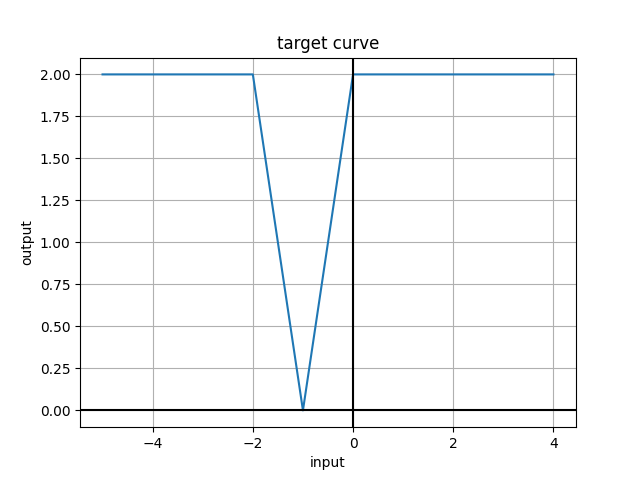
\includegraphics[width=0.8\textwidth]{part2/target-curve.png}
    \caption{Σύγκριση επιθυμητής έξοδου και εξόδου νευρωνικού δικτύου}
\end{figure}
\clearpage
\section{Θέμα}

Δεν απαντήθηκε.

\end{document}
